\section{Specification- and Syntax-based Linguistic Capability Testing}
%% \label{sec:approach}

\begin{figure*}
  \centering
  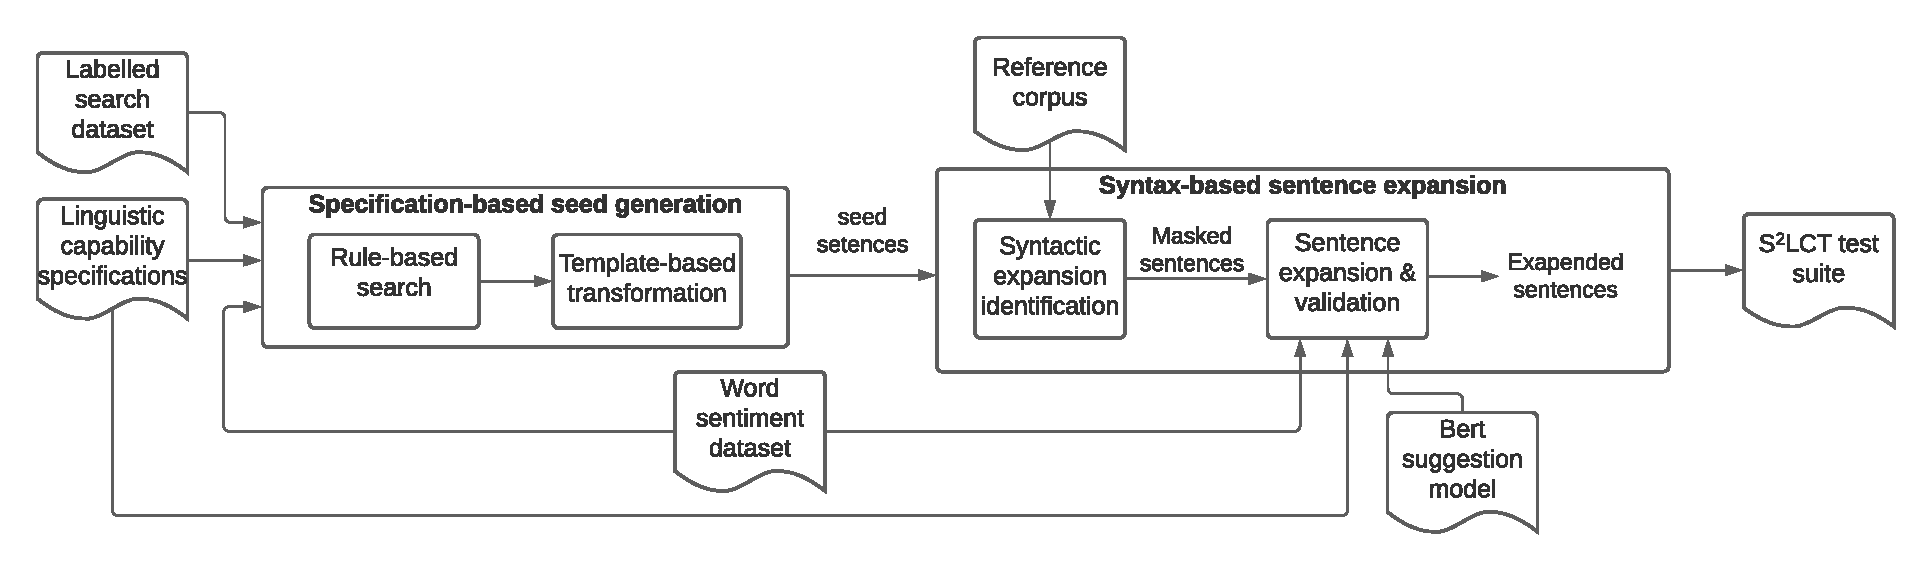
\includegraphics[width=\linewidth]{figs/overview.pdf}
  \caption{\OverviewFigCaption}
\end{figure*}

\sw{Some paragraphs in this overview part should go earlier in the
  paper. I am just writing them here for now as I don't think we have
  them in the intro/background yet.}  We design and implement
\emph{Specification- and Syntax-based Linguistic Capability Testing
  (\tool{})} to automatically generate test cases to test the
robustness of sentiment analysis models. We identify four goals for a
large and effective test suite:

\begin{description}
\item[{\bf G1}] the test suite should contain realistic sentences;
\item[{\bf G2}] the test suite should cover diverse syntactic structures;
  \item[{\bf G3}] each test case should be
categorized into a linguistic capability;
\item[{\bf G4}] the label of each test case should be
automatically and accurately defined.
\end{description}

\Chlst's templates generate complete and realistic sentences, and each
template maps to a linguistic capability, satisfying {\bf G1} and {\bf
  G3}. But \Chlst only uses \sw{X} manually created templates to
generate its test suite; all test cases generated by the same template
share the same syntactic structure, thus violating {\bf G2}. In
addition, the label of each \Chlst test case has to be decided
manually, associated with each template, violating {\bf G4}.

We present \tool{}, a new linguistic capability test case generation
tool, that satisfies all of these criteria.  \sw{I could not summarize
  a cohesive idea that drives our design. Leaving it here to fill in.
  Also, I felt my writing below still lacks justification for some
  design choices (e.g., why we do the differentiation).}
Figure~\ref{fig:overview} shows the overview of \tool{}, which
consists of two phases.  The \emph{specification-based seed
  generation} phase performs rule-based searches from a real-world
dataset ({\bf G1}) and template-based transformation to obtain the
initial seed sentences.  The search rules (e.g., search for neutral
sentences that do not include any positive or negative words) and
transformation templates (e.g., \sw{add an example} \jl{sentence
  negation}) are defined in the \emph{linguistic capability
  specifications}, which guarantee that each resulting seed conforms
to a specific linguistic capability ({\bf G3}) and is labelled
correctly ({\bf G4}).

The \emph{syntax-based sentence expansion} phase expands the seed
sentences with additional syntactic elements (i.e., words
\sw{more?}\jl{and production ruls in \cfg}) to cover many real-world
syntactic structures ({\bf G2}). It first performs a syntax analysis
to identify the part-of-speech (PoS) tags that can be inserted to each
seed, by comparing the PoS parse trees between the seed sentence and
many other sentences from a large reference dataset. Each identified
tag is inserted into the seed as a \emph{mask}. It then uses an NLP
recommendation model (i.e., BERT \cite{}) to suggest possible
words. If a resulting sentence is validated to be consistent with the
specification which additionally defines the rules for expansion
(e.g., the expanded word should be neutral), {\bf G3} and {\bf G4} are
still satisfied.  Last, because some validated sentences may include
unacceptable suggested words given the context \sw{is this the
  right motivation to do selection?} \jl{I edited the sentence. please
  let me know if it is clear}, we use a heuristic (i.e., the
confidence score from the NLP recommendation model) to select the more
realistic context-aware expanded sentences into \tool{}'s test suite.

We now describe each phase of \tool{} in detail.

%\Model generates input \sents with the following phases illustrated
%in \ref{fig:OverallModel}: 1. search phase searches seed \sents
%according to its \req of \lc, 2. seed parsing phase parses the found
%seed \sents and extract their \cfg, 3. reference parsing phase
%collects \pcfg from large corpus, 4. production differentiation phase
%identifies structural expansion candidates for input expansion, and
%5.\sent selection phase generates natural expanded \sent. In this
%section, we provide more details on each phase.

\subsection{Specification-based Seed Generation}
The seed generation phase of \tool starts by searching sentences in a
real-world dataset that match the rules defined in the linguistic
capability specification, and then transforming the matched sentences
using templates to generate seed sentences that conform to individual
linguistic capabilities. The reasons for this design choice are
twofold.  First, while generally judging which linguistic capability
any sentence falls into and which label it should have is infeasible,
there exist simple rules and templates to allow classifying the
resulting sentences into individual linguistic capabilities and with
the correct labels, with high confidence.  This enables us to test
each linguistic capability individually.  Second, searching from a
real-world dataset ensures that the sentences used as test cases for
testing linguistic capabilities are realistic and diverse. The diverse
test cases are more likely to achieve a high coverage of the target
model's functionality in each linguistic capability, thus detecting
more errors.

%The search phase in \Model searches inputs in dataset and selects
%subset of input \sents in the dataset that meets the \lc
%\req. The idea behind this phase is that input distribution of
%\lc is important to generate inputs relevant to \lc. \Lc explains
%expected behaviors of NLP model on specific types of input and
%output. The NLP model is evaluated on how much it performs on the
%input and output. Thus, \lc introduces the constraints of the input
%data. Input data from the constrained distribution are only qualified
%to be used for evaluating the NLP model on the \lc.  In addition,
%diversity in inputs is important to evaluate NLP models on the
%\lc. Inputs that differ are more likely to cover the NLP model
%behavior, and more coverage increases trustworthiness of the
%evaluation. To generate inputs from same distribution on \lc and high
%diversity of inputs, we estabilish \reqs of input and output
%for each \lc, and find inputs that fulfil the \reqs. Given a
%\lc, a \req consists of search \req, transform
%\req and expansion \req. The search \req
%describes features and functionalities that we seek to have in
%inputs. \Model check each input if it satisfy the \req.

Table \ref{tab:specification} shows the search rules and the
transformation templates of all 11 linguistic capabilities we
implemented in \tool{}. \sw{@Jaeseong: revise the rest of 3.1 based on
  Table \ref{tab:specification}. I commented out the old text but it
  is still in the tex file.}

\InputWithSpace{tables/lc-requirement-table}

%\begin{figure}[t]
%  \centering
%  \lstinputlisting[language=json-pretty]{code/requirement_sa1.json}
%  \vspace{-10pt}
%  \caption{\SearchRequirementExampleFigCaption}
%  \vspace{-10pt}
%\end{figure}
%
%\begin{figure}[t]
%  \centering
%  \subfloat[][\TransformRequirementExampleSubFigCaption]{\lstinputlisting[language=json-pretty]{code/requirement_sa2.json}}
%  \\
%  \subfloat[][\TransformTemplateExampleSubFigCaption]{\lstinputlisting[language=python]{code/requirement_sa2.py}}
%  \\
%  \caption{\TransformRequirementExampleFigCaption}
%  \vspace{-10pt}
%\end{figure}
%
%Figure~\ref{fig:SearchReqEx} shows \lc of \SareqExOne. To evaluate
%this \lc, the input is required to be short and have only \neu \adjs,
%\neu \nns. In addition, the label needs to be \neu. Therefore, all
%short natural \sents with only \neu \adjs and \neu \nns are available
%to evaluate NLP models. In this work, the sentiment of the words for
%the search are classified based on the sentiment scores from
%\Swn~\cite{baccianella2010sentiwordnet}, a publicly available English
%sentiment lexicons.  It provides lexical sentiment scores and the
%sentiment word labels are categorized by implementing the rules
%in~\cite{mihaela2017sentiwordnetlabel}. Next, transform \req explains
%how the input and output needs to be tranfromed. Some \lc only accepts
%heavily limited input distribution, and it is unlikely to be included
%in searching dataset because of its high structural diversity, thus,
%finding such \sents is costly. Therefore, our approach is to find
%inputs by relaxing search requirement and transform the input to match
%the target requirement of the \lc. In this work, the inputs are
%transformed by word addition or perturbing the found inputs with \lc
%dependent templates. The figure~\ref{fig:TransformReqEx} shows the
%example of use of the template requirement. The \lc of \SareqExTwo in
%the figure~\ref{fig:TransformReqSubEx} requires inputs to be the
%negated \pstv \sents and the neutral expression in the middle. Rather
%than searching \sents that match the input distribution of the \lc,
%the \Model search \pstv and \neu inputs and combine them into negated
%\pstv \sents. Figure~\ref{fig:TransformTempSubEx} illustrates template
%for the \lc. According to the \lc, The value of ``sent1'' and
%``sent2'' become each searched \neu and \pstv inputs respectively, and
%the template completion generates new inputs that matches the target
%\lc. In addition, the transformation of inputs also produce high
%diversity in the inputs because of that from initially found
%inputs. In this paper, we will denote the searched inputs in this
%phase as seed inputs.

\subsection{Syntax-based Sentence Expansion}

The simple search rules and transformation templates used to generate
the seed sentences may limit the syntactic structures these seeds may
cover. To address this limitation, the syntax-based sentence expansion
phase extends the seed sentences to cover syntactic structures
commonly used in real-life sentences. Our idea is to differentiate the
parse trees between the seed sentences and the reference sentences
from a large real-world dataset. The extra PoS tags in the reference
parse trees are identified as potential syntactic elements for
expansion and inserted into the seed sentences as masks. We then use
masked language model to suggest the fill-ins. If the resulting
sentences still conform to the linguistic capability specification,
they are added to \tool{}'s test suite. \sw{May have some redundancy
  and inconsistency with the overview part.}

\subsubsection{Syntax Expansion Identification}

Algorithm \ref{alg:diff} shows how masks are identified for each seed
sentence.  It takes the parse trees of the seeds, generated by the
Berkeley Neural
Parser~\cite{kitaev2018seedparser,kitaev2019seedparser}, and a
reference context-free grammar (CFG) from the Penn Treebank corpus
dataset \cite{} as inputs.  The reference CFG is learned from a large
dataset \cite{} that is representative of the distribution of
real-world language usage.  The algorithm identifies the discrepancy
between the seed syntax and the reference grammar to decide how a seed
can be expanded.
%This phase builds \pcfg from the reference corpus. \cfg
%is constructed by parsing sentences in the corpus and extracting
%\prodrs. In addition, the probability of \cfg is estimated by
%its frequency over corpus. The output of this phase is the constructed
%\pcfg, and it is compared with seed parse trees. For our
%implementation, we build the \pcfg from the Penn Treebank corpus dataset.


%\paragraph{Seed parsing.}
%To expand seed sentence and generate fluent and faithful sentence
%used for evaluation, \Model studies structure of each seed input for
%its expansion.
%Seed parsing takes each seed as
%input, and outputs its parse tree of the seed, using the Berkeley Neural
%Parser~\cite{kitaev2018seedparser,kitaev2019seedparser}.

%\paragraph{Reference parsing.}
%We take a large-scale real-world dataset as reference for sentence expansion.

\begin{algorithm}
  \caption{\ProdDiffAlgCaption}
  \begin{algorithmic}[1]
    \State \textbf{Input:} Parse trees of seed sentences $\textbf{S}$,
    reference \pcfg$\textbf{R}$
    \State \textbf{Output:} Set of expanded masked sentences $\textbf{S\_exp}$
    \For {$seed$ from $S$}
      \For {each production rule $seed\_prod$ from $seed$}
        \State $seed\_lhs = seed\_prod.lhs$
        \State $seed\_rhs = seed\_prod.rhs$
        \For {$ref\_rhs$, $ref\_prob$ from $R[seed\_lhs]$}
          \If {$seed\_rhs$ is superset of $ref\_rhs$}
            \State $parent = seed\_prod.parent$
            \State $prob = ref\_prob$
            \While {$parent$ is not empty}
              \For {$par\_rhs$, $par\_prob$ from $R[parent.lhs]$}
                \If {$parent.rhs == par\_rhs$}
                  \State $prob = prob \cdot par\_prob$
                  \State $parent = parent.parent$
                  \State break
                \EndIf
              \EndFor  
            \EndWhile
            \State $P.add([seed\_prod, ref\_prod, prob])$
          \EndIf
        \EndFor
      \EndFor
      \If {$P$ is not empty}  
        \State Select Top-k $ref\_prod$ along with probabilities in P
        \For {each $seed\_prod$, $ref\_prod$ in the Top-k selected P}
          \State replace $seed\_prod$ with $ref\_prod$ in $seed$
          \State replace expanded component in $ref\_prod$ with $MASK$
          token in $seed$ sentence
          \State $S\_exp.add([ref\_prod, expanded sentence])$
        \EndFor
      \EndIf
    \EndFor
  \end{algorithmic}
\end{algorithm}


For each production of in each seed's parse tree (lines 3 and 4), we
extract its non-terminal at the left-hand-side (line 5), $s\_lhs$, and
the grammar symbols at the right-hand-side (line 6), $s\_rhs$. In line
7, the algorithm iterates through all productions in the reference
context-free grammar and match these that have the same non-terminal
at the left-hand-side as $s\_lhs$.  The right-hand-side of each
matched production is called $r\_rhs$.  If $s\_rhs$ consists of a
subset of the grammar symbols in $r\_rhs$ (line 8), the additional
symbols in the $r\_rhs$ are inserted as masks in the parse tree of
seed sentence, in their respective positions in the expanded
production.  The left to right traversal of the leaves of an expanded
parse tree forms a masked sentence.  Lastly, we randomly select $k$
masked sentences for the next sentence expansion and validation phase.
\sw{Add justification: why we need to select k masked sentences
  (performance?) and why random makes sense.}

\begin{figure*}[t]
  \centering
  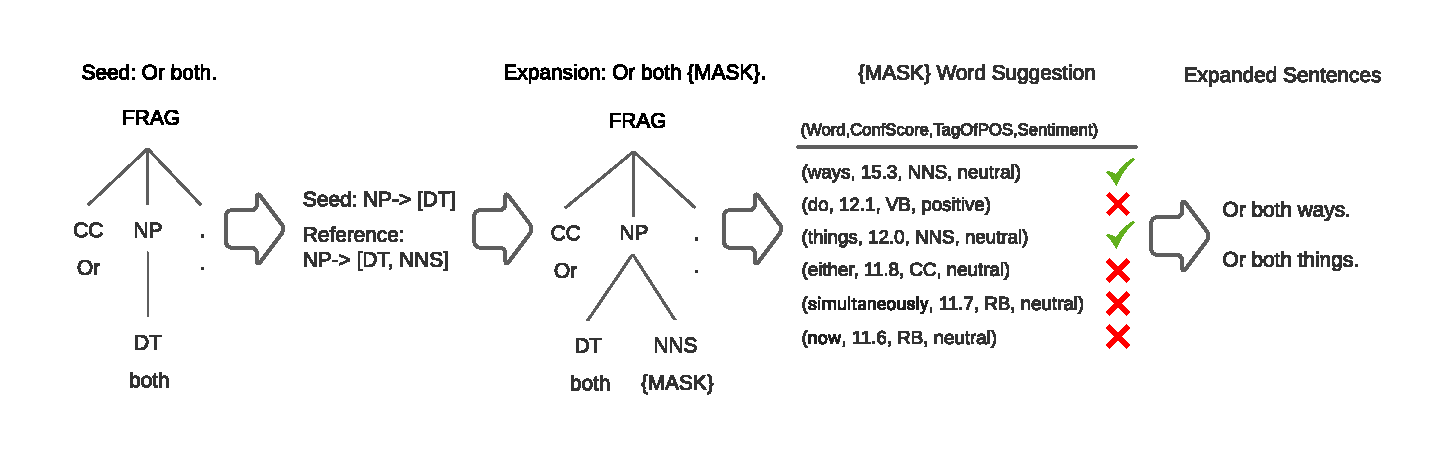
\includegraphics[scale=0.7]{figs/running_example.pdf}
  \caption{\RunningExCaption}
%  Expansion of the seed sentence ``Or
%both.''. For a \prodr in seed ``NP->[DT]'' on the left, the \prodr of
%``NP->[DT, NNS]'' is found in reference. Thus, the component NNS can be expanded in the
%seed and ``NP->[DT]'' is replaced with ``NP->[DT, NNS]'' and it generates new
%expanded sentence on the right.
\end{figure*}

\paragraph{Running example.} Figure~\ref{fig:ExpEx} shows an example using Algorithm \ref{alg:diff}
to generate a masked sentence. The sentence ``Or both." is a seed of
\sw{which?} linguistic capability.  The tree on the left shows the
parse tree of this seed; it consists of two productions: ``FRAG->[CC,
  NP, .]" and ``NP->[DT]".  When matching the left-hand-side
non-terminal of the second production (i.e., ``NP") in the reference
CFG, we found that it includes a production ``NP->[DT, NNS]" which has
an additional symbol ``NNS" on the right-hand-side.  The algorithm
thus expands the parse tree with this symbol, shown in the second
tree.  The masked sentence ``Or both \{MASK\}." is the result of the
left-to-right traversal of this expanded parse tree.

%Given the seed parse tree and reference \pcfg, production
%differentiation phase suggests structural expansion candidates on the
%seed input. this phase aims to analyze which structural components and
%where they can be added into the seed structure for its expansion. To
%do so, we explore reference \prodrs comparing it with each \prodr used
%in seed input. This results in the phase described in
%Algorithm~\ref{code:ProdDiffAlg}. For each production rule in seed
%inputs ($seed\_prod$), it searches production rules in reference
%($ref\_prod$) which it has same non-terminal on the \lhs
%($seed\_prod.lhs==ref\_prod.lhs$) and superset of \rhs of the seed
%production rule ($seed\_prod.rhs \subset ref\_prod.rhs$).  As we
%assume that the reference \cfg is built from real world data
%distribution, the elements in the complement set ($ref\_prod.rhs -
%seed\_prod.rhs$) become an expansion candidate which can be expanded
%from the $seed\_prod.rhs$ found in real world. In addition, the
%measure of how consistent the production rule is with the given seed
%structure is given in its probability of the reference production rule
%($ref\_prob$) multiplied by that of parents of $seed\_prod$. The
%expansion candidate consists of terminal or nonterminal symbols. When
%there is a phrase-level or clause-level nonterminal symbol, \eg noun
%phrase, it needs to be expanded and replaced with word-level
%nonterminal or terminal symbols to generate the expansion
%candidate. The number of feasible replacement is unbounded because of
%its high degree of freedom. Therefore, in this work, we focus on the
%expansion candidate with only the word-level nonterminal or terminal
%symbols for the effectiveness of \Model. Lastly, the expanded
%component is replaced with the mask token for the next phase. The
%example of the expansion is illustrated in
%Figure~\ref{fig:ExpEx}. The ``NP->[DT]'' is queried into
%reference, and ``NP->[DT,NNS]'' is identified as its expansion
%candidate since the \rhs of ``NP->[DT,NNS]'' is superset of that of
%``NP->[DT]''. the component of NNS is replaced with mask token in
%sentence-level. Therefore, the ``Or both \{MASK\}.'' is suggested for
%the next phase.

\subsubsection{Sentence Expansion and Validation}

In this phase, the words to fill in the masks in the masked sentences
are suggested by the BERT pretrained model \cite{}.  The BERT model
suggests word for the mask symbol

according to its context \sw{what does context mean here?} around in
sentence.  \sw{Algorithm 1 does not require we only have one mask in
  the masked sentence. Can the model suggest multiple words at the
  same time?}  \sw{Say a bit more about the BERT model
  suggestion. E.g., it may suggest multiple words for the same mask
  but they are ranked?}

Because BERT model is not aware of the linguistic capability
specification and the grammar symbol in the expanded parse tree, an
expanded sentence using the suggested words may no longer satisfy the
linguistic capability specification. Therefore, we perform validation
on the suggested words and only accept them if the following three
criteria are met.

First, the PoS tag of the suggested word must match the PoS tag of the
expanded symbol in the parse tree. For the example in
Figure~\ref{fig:ExpEx}, the masked symbol is a ``NNS" (i.e., plural
noun); thus, the suggested word must also be a ``NNS". \sw{Say how we
  obtain the PoS tag of a suggested word.}  Second, we require that
the sentiment of the expanded sentence is the same as the seed
sentence. To ensure this, the suggested words must be neutral.
\sw{Should we present this as part of specification, called expansion
  rule?}  Third, we additionally verify that the expanded sentences
satisfied the same search rules for the seed sentence. Our goal for
generating the expanded sentences is to use them for evaluating the
\sa models on the associated \lc in addition to the seed sentence. It
is only achieved when the expanded sentences are also met with the
same search rules for the \lc. For LC1 as an example, the expanded
sentence must still conform to the specification of the seed's
linguistic capability specification. Therefore, the expanded sentences
are required to be short and to only have neutral adjectives and
nouns. \sw{Say why we use the third criteria only for LC1 and LC2.}
\jl{I added the explanation}

\paragraph{Running example.} The third step in Figure~\ref{fig:ExpEx} shows the words suggested
by BERT. For this masked sentence, BERT suggested six words. Each word
is associated with the confidence score provided by BERT, the PoS tag,
and the sentiment. Among the six words, only ``ways'' and ``things''
are validated by \tool{} because they have the Pos tag ``NNS'' and are
neutral. In addition, it is found that both sentences meets the search
rule of the associated \lc of \SareqExOne. In the end, two sentences
of ``Or both ways'' and ``Or both things'' are generated.  \sw{Do we
  also check if the expanded sentence meets the
  specification?}\jl{Yes. I added the explanation of validation of \lc
  \req}

%The suggested word are
%validated by three criteria. First, The tag of POS must be matched with
%that suggested from the production differentiation phase. In the
%example in the Figure~\ref{fig:ExpEx}, the mask token comes from the
%structural component of NNS, plural noun. Therefore, the BERT
%suggested words must be also tagged with the NNS. Accordingly, every
%words of the NNS are only available. Second, \Model focuses on the \sa
%task, and it assume that the suggested words must not change sentiment
%of its input and must preserve its consistency of original sentiment
%label. Therefore, we only accept the \neu words for the
%expansion. Third, the expanded sentences with the BERT suggested words
%must be appropriate for evaluating NLP models on the target \lc, and the
%sentences must pass the \req of the \lc. In this work, the BERT
%suggestions are validated by the three criteria.

\subsubsection{Sentence Selection}
\sw{@Jaeseong: Add how we select expanded sentences and motivate why.}
After 
\paragraph{Running example.} \sw{Refer to the example to say how we
  use the BERT score to select.} \jl{I dont think we need this
  subsection of sentence selection it is already explained at the
  previous stage with running example.}
